\documentclass[a4paper, 12pt]{article}

\author{%
    b13701220 顧懷允,
    b13703048 林子宸,
    b13705036 劉威廷,
    b13303079 闕以諾
}
\title{\textbf{Operations Research\\Midterm Project}}
\date{May 2026}

\usepackage[margin=2.3cm]{geometry}
\usepackage{amsmath}
\usepackage{amssymb}
\usepackage{amsthm}
\usepackage{enumitem}
\usepackage{graphicx}
\usepackage{listings, lstautogobble}
\usepackage{booktabs}
\usepackage{float}

\usepackage{tabularray}
\UseTblrLibrary{amsmath, siunitx}

\usepackage{tikz}

\usepackage{xeCJK}
\setCJKmainfont{Heiti TC}

\graphicspath{{./}}

\setlist{nosep}

\begin{document}
    \maketitle

\section{Problem Description and Notation}

The IEDO company operates $n_S$ stations, $n_C$ cars across $n_L$ levels, and books $n_K$ orders over an $n_D$-day horizon. Each order $k$ specifies a requested level $\ell_k$, a pickup station/time $(s^p_k, t^p_k)$, a return station/time $(s^r_k, t^r_k)$, and a revenue $R_k = F_{\ell_k}\cdot H_k$. The company decides (i) which orders to accept, (ii) which car serves each accepted order---possibly via a one-step \emph{upgrade} (a level-$\ell$ order may be served by a level-$\ell$ or level-$(\ell{+}1)$ car), and (iii) when and where employees relocate cars. Accepting order $k$ earns $R_k$; rejecting it costs $2R_k$. The objective is to maximize total profit.

\smallskip
\noindent\textbf{Operating rules.} After a car is returned, IEDO assumes a 1\,h late buffer plus a 3\,h cleaning, so the car becomes \emph{ready} $\Theta := 240$ min after the scheduled return time at its return station. A car must be at the pickup station at least $\Delta := 30$ min before pickup. Cars may be relocated between stations $i$ and $j$ in $T_{ij}$ minutes (symmetric, $T_{ii}{=}0$, multiple of 30). The sum of relocation minutes over all employee-driven moves is bounded by $B$. All cars are considered ready at the origin of the planning horizon.

\smallskip
\noindent\textbf{Common notation} (used in \S\ref{sec:milp}--\S\ref{sec:p4}).

\begin{center}
\begin{tblr}{
  colspec = {l X[l]},
  rowsep = 1pt,
  row{1} = {font=\bfseries},
}
Symbol & Meaning \\
\hline
$S,\,C,\,K$ & sets of stations, cars, and orders \\
$\ell_c,\,s^0_c$ & level and initial station of car $c$ \\
$\ell_k,\,s^p_k,\,s^r_k,\,t^p_k,\,t^r_k,\,R_k$ & level, pickup/return station, pickup/return time (min from 2023/01/01 00:00), revenue of order $k$ \\
$T_{ij}$ & relocation time (min) between stations $i$ and $j$, symmetric \\
$B$ & total relocation-time budget (min) \\
$\Delta = 30,\;\Theta = 240$ & pickup-lead time and post-return-ready buffer (min) \\
$\mathrm{lvl}(c,k)$ & predicate $\ell_k \le \ell_c \le \ell_k + 1$ (car $c$ may serve order $k$, possibly as an upgrade) \\
\end{tblr}
\end{center}


\section{Problem 1: Mixed-Integer Programming Model}\label{sec:milp}

We formulate the planning problem as a per-car path-flow MILP on a time-feasibility DAG. Each car traces an ordered (possibly empty) sequence of orders from a virtual source (its initial station at time 0) to a virtual sink. An arc exists between two orders only if a single car can serve them consecutively under the cleaning, lead-time, and level rules.

\subsection{Feasibility-filtered index sets}

\begin{align*}
\mathcal{V}^{\text{src}} &= \bigl\{ (c,k)\in C\times K : \mathrm{lvl}(c,k),\;\; T_{s^0_c,\,s^p_k}\le \max(0,\;t^p_k - \Delta)\bigr\}, \\
\mathcal{V}^{\text{chn}} &= \bigl\{ (c,i,j)\in C\times K\times K : i\ne j,\; \mathrm{lvl}(c,i),\; \mathrm{lvl}(c,j),\;\; t^r_i + \Theta + T_{s^r_i,\,s^p_j} \le t^p_j - \Delta\bigr\}, \\
\mathcal{V}^{\text{snk}} &= \bigl\{ (c,k)\in C\times K : \mathrm{lvl}(c,k)\bigr\}.
\end{align*}
Restricting variables to these sparse sets dramatically reduces model size and is enough to encode every operational rule: source feasibility encodes the initial-position lead-time constraint (with the $\max(0,\,\cdot)$ accounting for the problem's assumption that all cars are ready at the origin and may be picked up immediately at $t=0$ from their home station, in which case the $\Delta$ lead-time is waived); chain feasibility encodes the cleaning, ready-buffer, relocation, and lead-time rules in one inequality.

\subsection{Decision variables}

\begin{itemize}
\item $x^{\text{src}}_{c,k}\in\{0,1\}$ for $(c,k)\in\mathcal{V}^{\text{src}}$: car $c$ starts its tour by serving order $k$.
\item $x^{\text{chn}}_{c,i,j}\in\{0,1\}$ for $(c,i,j)\in\mathcal{V}^{\text{chn}}$: car $c$ serves $i$ then immediately $j$.
\item $x^{\text{snk}}_{c,k}\in\{0,1\}$ for $(c,k)\in\mathcal{V}^{\text{snk}}$: car $c$ ends its tour at order $k$.
\item $y_k\in\{0,1\}$: order $k$ is accepted.
\end{itemize}

\subsection{Constraints}

\textbf{(C1) At most one source per car.} A car either sits idle or starts exactly one tour:
\[
\sum_{k:\,(c,k)\in\mathcal{V}^{\text{src}}} x^{\text{src}}_{c,k} \;\le\; 1, \qquad \forall c\in C.
\]

\textbf{(C2) Flow conservation at every (car, order) node.} For every $(c,k)$ with $\mathrm{lvl}(c,k)$,
\[
\underbrace{x^{\text{src}}_{c,k} \cdot \mathbb{1}[(c,k)\in\mathcal{V}^{\text{src}}] + \sum_{i:\,(c,i,k)\in\mathcal{V}^{\text{chn}}} x^{\text{chn}}_{c,i,k}}_{\text{flow into node }(c,k)}
\;=\;
\underbrace{x^{\text{snk}}_{c,k} + \sum_{j:\,(c,k,j)\in\mathcal{V}^{\text{chn}}} x^{\text{chn}}_{c,k,j}}_{\text{flow out of node }(c,k)}.
\]

\textbf{(C3) Acceptance links flow to $y$.} Each accepted order is served by exactly one car:
\[
\sum_{c\in C}\Biggl(x^{\text{src}}_{c,k}\cdot \mathbb{1}[(c,k)\in\mathcal{V}^{\text{src}}] + \sum_{i:\,(c,i,k)\in\mathcal{V}^{\text{chn}}} x^{\text{chn}}_{c,i,k}\Biggr) \;=\; y_k, \qquad \forall k\in K.
\]

\textbf{(C4) Relocation budget.} Only positive-distance arcs consume budget:
\[
\sum_{(c,k)\in\mathcal{V}^{\text{src}}} T_{s^0_c,\,s^p_k}\, x^{\text{src}}_{c,k} \;+\; \sum_{(c,i,j)\in\mathcal{V}^{\text{chn}}} T_{s^r_i,\,s^p_j}\, x^{\text{chn}}_{c,i,j} \;\le\; B.
\]

\subsection{Objective}

The IEDO profit is
\[
\max\; \sum_{k\in K} R_k\, y_k \;-\; 2\sum_{k\in K} R_k\,(1-y_k) \;\equiv\; 3\sum_{k\in K} R_k\, y_k \;-\; 2\sum_{k\in K} R_k,
\]
where the second form drops the additive constant for solver efficiency. The model is a pure binary program. Acyclicity of the chain DAG (times are strictly increasing along any feasible chain) precludes subtours, so no extra cuts are needed.


\section{Problem 1: Optimal Plan for Instance 5}\label{sec:instance5}

Solving the MILP of \S\ref{sec:milp} on \texttt{instance05.txt} with Gurobi (Python~3.12, default settings) yields the provably optimal profit \textbf{NT\$\,106{,}800} in well under one second. Below we present the plan in operational language.

\subsection{Headline}

\begin{center}
\begin{tblr}{
  colspec = {X[l] r},
  rowsep = 1pt,
  row{1} = {font=\bfseries},
}
Item & Amount (NT\$) \\
\hline
Sales revenue from the 8 accepted orders & 117{,}000 \\
Compensation paid to the 2 rejected customers ($2\times$ revenue) & 10{,}200 \\
\textbf{Net profit} & \textbf{106{,}800} \\
\end{tblr}
\end{center}

\noindent We accept 8 of 10 orders, decline 2, perform 1 free upgrade, and use 1{,}080 of the 1{,}200 budgeted relocation minutes (90\%). No feasible alternative plan does strictly better.

\subsection{Order-by-order decision}

\begin{center}\small
\begin{tblr}{
  colspec = {c c l l r l c c},
  rowsep = 1pt,
  colsep = 4pt,
  row{1} = {font=\bfseries},
}
Order & Lv & Pickup & Return & Rev. & Decision & Car & Upg.\\
\hline
1  & 1 & St.1, Day4 01:00 & St.6, Day4 20:00 &  1{,}900 & Reject ($-3{,}800$) & --- & --- \\
2  & 1 & St.4, Day1 16:00 & St.5, Day3 00:00 &  3{,}200 & Reject ($-6{,}400$) & --- & --- \\
3  & 1 & St.5, Day2 03:30 & St.1, Day4 11:30 &  5{,}600 & Accept & 3 & No \\
4  & 1 & St.1, Day3 12:00 & St.2, Day5 15:00 &  5{,}100 & Accept & 1 & No \\
5  & 2 & St.6, Day1 00:00 & St.6, Day4 20:00 & 36{,}800 & Accept & 6 & No \\
6  & 1 & St.3, Day4 23:00 & St.4, Day5 14:00 &  1{,}500 & Accept & 4 & \textbf{Yes} \\
7  & 2 & St.2, Day2 03:30 & St.1, Day4 23:30 & 27{,}200 & Accept & 5 & No \\
8  & 2 & St.6, Day5 04:30 & St.6, Day5 14:30 &  4{,}000 & Accept & 6 & No \\
9  & 2 & St.3, Day1 19:30 & St.4, Day4 15:30 & 27{,}200 & Accept & 4 & No \\
10 & 1 & St.4, Day1 06:00 & St.2, Day5 06:00 &  9{,}600 & Accept & 2 & No \\
\end{tblr}
\end{center}

\noindent\emph{Why decline?} Orders 1 and 2 are small-revenue level-1 jobs whose pickup windows collide with strictly more lucrative commitments: serving them would force the cancellation of orders 4/10 or 7/9 (which together earn over NT\$\,69{,}000). Paying NT\$\,10{,}200 in compensation is cheaper than that opportunity cost. \emph{Free upgrade.} Order 6 (level-1) is most profitably satisfied by the level-2 Car 4, which has just completed Order 9 and sits at a convenient station.

\subsection{Relocation work orders}

Five employee-driven moves, totalling 1{,}080 of the 1{,}200 budgeted minutes:

\begin{center}
\begin{tblr}{
  colspec = {c c c c l l r},
  rowsep = 1pt,
  row{1} = {font=\bfseries},
}
\# & Car & From & To & Depart & Arrive & Duration \\
\hline
1 & 2 & St.2 & St.4 & Day1 01:30 & Day1 05:30 & 240 \\
2 & 4 & St.5 & St.3 & Day1 15:30 & Day1 19:00 & 210 \\
3 & 5 & St.4 & St.2 & Day1 23:00 & Day2 03:00 & 240 \\
4 & 3 & St.3 & St.5 & Day1 23:30 & Day2 03:00 & 210 \\
5 & 4 & St.4 & St.3 & Day4 19:30 & Day4 22:30 & 180 \\
\hline
  &   &      &      &            & Total      & \textbf{1{,}080} / 1{,}200 \\
\end{tblr}
\end{center}

\subsection{Per-car schedules}

\begin{itemize}
\item \textbf{Car 1} (L1, st.1): Order 4 only [pick St.1 Day3 12:00 $\to$ ret St.2 Day5 15:00]. No relocation.
\item \textbf{Car 2} (L1, st.2): Relocate St.2$\to$St.4 (Day1 01:30, 240 min) $\Rightarrow$ Order 10 [Day1 06:00 $\to$ Day5 06:00 St.2].
\item \textbf{Car 3} (L1, st.3): Relocate St.3$\to$St.5 (Day1 23:30, 210 min) $\Rightarrow$ Order 3 [Day2 03:30 $\to$ Day4 11:30 St.1].
\item \textbf{Car 4} (L2, st.5): Relocate St.5$\to$St.3 $\Rightarrow$ Order 9 [Day1 19:30 $\to$ Day4 15:30 St.4]; ready Day4 19:30, relocate St.4$\to$St.3 $\Rightarrow$ Order 6 \emph{(upgrade)} [Day4 23:00 $\to$ Day5 14:00].
\item \textbf{Car 5} (L2, st.4): Relocate St.4$\to$St.2 $\Rightarrow$ Order 7 [Day2 03:30 $\to$ Day4 23:30 St.1].
\item \textbf{Car 6} (L2, st.6): Order 5 [Day1 00:00 $\to$ Day4 20:00 St.6]; ready Day5 00:00 $\Rightarrow$ Order 8 [Day5 04:30 $\to$ Day5 14:30 St.6]. No relocation.
\end{itemize}


\section{Problem 2 \& 3: Heuristic Algorithm}\label{sec:heuristic}

While the MILP of \S\ref{sec:milp} solves Instance 5 in well under one second, on a larger instance (say $n_K = 10{,}000$) the chain-arc count is $\mathcal{O}(n_C \cdot n_K^2) \approx 10^{11}$, well beyond the three-minute budget. We therefore design a three-tier heuristic that recovers the exact MILP at small scales and degrades gracefully.

\subsection{Algorithm design}

To solve the car-rental scheduling problem across varying scales and ensure the program produces a feasible solution within the 3-minute limit, our algorithm adopts a \textbf{Three-Tier Adaptive Architecture}. The key idea is to use different strategies for different instance sizes. Small instances are solved by a Path-flow MIP (the model of \S\ref{sec:milp} with a tight solver time limit), medium-sized instances by a Revenue-first Insertion Heuristic, and large instances by a fast Heap-Based Chronological Greedy. This achieves a good balance between solution quality and computational efficiency.

\subsection{Algorithm structure}

\subsubsection*{Flow chart}
\begin{figure}[H]
    \centering
    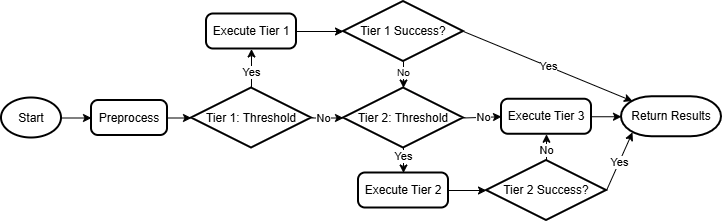
\includegraphics[width=0.88\linewidth]{OR_flowchart.png}
\end{figure}

\subsubsection*{Data preprocessing}
\begin{itemize}
    \item \textbf{Time cache.} Convert all string-formatted times into ``minutes elapsed since 2023/01/01 00:00.'' A dictionary cache avoids repeated string parsing, reducing I/O conversion cost on large instances.
    \item \textbf{Moving-time matrix.} Build a 2-D array \texttt{moving\_time[i][j]} so all relocation-time queries are $\mathcal{O}(1)$.
\end{itemize}

\subsubsection*{Tier 1: Small instances (Path-flow MIP)}
\begin{itemize}
    \item \textbf{Trigger:} $n_K \le 160$ and $n_C\cdot n_K^2 \le 700{,}000$.
    \item \textbf{Logic:} Build the path-flow MILP of \S\ref{sec:milp}. Decision variables $x_{c,i,j}$ encode whether car $c$, after serving order $i$, has enough cleaning and moving time to next serve $j$. Gurobi's time limit is set to 20 s; if solved successfully, return the optimal schedule directly.
\end{itemize}

\subsubsection*{Tier 2: Medium instances (Revenue-first Insertion Heuristic)}
\begin{itemize}
    \item \textbf{Trigger:} $n_K \le 6{,}000$ and $n_C\cdot n_K \le 600{,}000$.
    \item \textbf{Logic:} Driven by the intuition of ``maximize business profit.''
    \begin{enumerate}[label=\textbf{\alph*.}]
        \item Sort all orders in descending order of $R_k$.
        \item Process high-revenue orders first; search candidate cars satisfying the level rule (same level or free upgrade).
        \item Use binary search to attempt inserting the new order into the car's existing schedule (sorted by pickup time).
        \item Check the immediately previous and next orders at the insertion position to ensure no conflict after accounting for cleaning and moving times. Assign the car that consumes the least additional relocation budget.
    \end{enumerate}
\end{itemize}

\subsubsection*{Tier 3: Large instances (Heap-Based Chronological Greedy)}
\begin{itemize}
    \item \textbf{Trigger:} ultimate fallback when Tiers 1--2 time out or the instance is too large.
    \item \textbf{Logic:} simulate the passage of time in the real world.
    \begin{enumerate}[label=\textbf{\alph*.}]
        \item Maintain a min-heap for each (station, car-level) pair, keyed by ``earliest ready time.''
        \item Sort orders chronologically by pickup time.
        \item For each order in order, attempt to pop the earliest-ready car from the pickup station's heap in $\mathcal{O}(\log n_C)$.
        \item If no local car is available, scan a pre-built ``nearest-stations'' list, evaluate moving time and remaining budget, and relocate a car from a nearby station. After serving, update the ready time and push the car into the return station's heap.
    \end{enumerate}
\end{itemize}

\subsection{Time complexity}

Let $K = n_K, C = n_C, S = n_S, L = n_L$.

\smallskip
\noindent\textit{Preprocessing.} Building the moving-time matrix is $\mathcal{O}(S^2)$ and converting all order times is $\mathcal{O}(K)$:
\[ T_{\text{prep}} = \mathcal{O}(K + C + S^2). \]

\noindent\textit{Tier 1 MIP.} The main arc-creation loop is $\mathcal{O}(n_C\cdot n_K^2)$:
\[ T_{\text{MIP}} = \mathcal{O}(n_C\cdot n_K^2). \]

\noindent\textit{Tier 2 Insertion heuristic.}
\begin{itemize}
    \item Sort orders: $\mathcal{O}(n_K\log n_K)$.
    \item For each order, scan all candidate cars and binary-search the insertion position: $\mathcal{O}(n_C\log n_K)$.
    \item Actual insert: $\mathcal{O}(n_K)$ per insertion.
    \item Total: $T_{\text{insertion}} = \mathcal{O}(n_K\cdot n_C\cdot \log n_K + n_K^2)$.
\end{itemize}

\noindent\textit{Tier 3 Heap greedy.}
\begin{itemize}
    \item Precompute nearest-neighbour list: $\mathcal{O}(n_S^2\log n_S)$.
    \item Sort orders: $\mathcal{O}(n_K\log n_K)$.
    \item Process each order: local-station check $\mathcal{O}(n_L)$, cross-station scan $\mathcal{O}(\text{scan\_limit}\cdot n_L\cdot \log n_C)$.
    \item Total (large $n_S$): $T_{\text{greedy}} = \mathcal{O}(n_S^2\log n_S + n_K\cdot \sqrt{n_S}\cdot n_L\cdot \log n_C)$.
\end{itemize}

\section{Problem 4: Numerical Experiments}\label{sec:p4}

Five hand-crafted instances are too few to validate a \emph{three}-tier algorithm. To exercise every tier we run a $3\times 4$ factorial: three \emph{blocks} (sized to fire Tier 1 / 2 / 3 respectively, see \S\ref{sec:heuristic}) crossed with four \emph{scenarios} (baseline, skewed-level demand, imbalanced spatial flow, high-demand load). Each (block, scenario) cell holds 25 random instances at Tier 1--2 and 15 at Tier 3 (260 total).

\subsection{Factors, scenarios, instance generation}

\begin{center}\small
\begin{tblr}{
  colspec = {l c c c c c X[l]},
  rowsep = 1pt,
  row{1} = {font=\bfseries},
}
Block & $n_S$ & $n_C$ & $n_K$ & $n_D$ & $B$ & Tier fired by heuristic \\
\hline
A (Small)  &  4 &   6 & 18\,/\,28   &  3 &    900 & Tier 1 — path-flow MIP \\
B (Medium) &  8 &  20 & 200\,/\,300 &  5 &  4\,000 & Tier 2 — insertion heuristic \\
C (Large)  & 20 & 200 & 7\,000\,/\,10\,000 & 10 & 20\,000 & Tier 3 — heap greedy \\
\end{tblr}
\end{center}

Within each block, four scenarios isolate one factor at a time: \emph{baseline} (everything uniform), \emph{skewed levels} ($\ell_k\sim(0.6,0.3,0.1)$ over $\{1,2,3\}$), \emph{imbalanced flow} (stations split into two groups; pickup biased to one, return to the other), and \emph{high demand} (the second value of $n_K$ above). Shared settings: $(F_1,F_2,F_3)=(200,300,500)$\,NT\$/h; $H_k\!\in\!\{2,3,4,6,8,12,18,24\}$\,h; $T_{ij}\!\in\!\{30,\!\dots\!,180\}$\,min, symmetric.

\subsection{Benchmarks and gap metrics}\label{sec:p4-method}

\textbf{Exact MIP optimum} $\pi^{\ast}$. Available only for Block A: at medium / large scales the path-flow MILP has $\gtrsim\!10^5$ binary variables, far beyond what our Gurobi licence will build. \textbf{LP-relaxation upper bound} $\pi^{\mathrm{UB}}$, always computable. For each 30-minute bucket $t$ and each level threshold $L\!\in\!\{1,\!\dots\!,n_L\}$ we add
\[
    \sum_{k\,:\,t\in[t^p_k,t^r_k),\;\ell_k\ge L} y_k \;\le\; \sum_{c\ge L} n_{C,c},
    \qquad y_k\in[0,1],
\]
i.e.\ at any time, simultaneously active orders at level $\ge L$ cannot exceed the cars at level $\ge L$ (a strict relaxation since cleaning, lead-time, station capacity, and relocation budget are all dropped). This is a small LP ($n_K$ vars, $\le n_L\cdot 480$ constraints), solved by HiGHS in $<\!1$\,s even when $n_K\!=\!10\,000$. It is loose at tight scales but provably valid. \textbf{Naive greedy} $\pi^{\mathrm{g}}$: chronological scan; first eligible car at the pickup station, relocate only if no local car works.

Because $\pi$ can be negative we use worst-case-normalised gaps
\[
    \mathrm{Gap}(\pi\,;\,\mathrm{ref}) = \frac{\mathrm{ref} - \pi}{\mathrm{ref} - L} \in [0,1],
    \qquad L = -2\!\sum_{k}\! R_k,
\]
where $\mathrm{ref}\!=\!\pi^{\ast}$ for Block A and $\mathrm{ref}\!=\!\pi^{\mathrm{UB}}$ for Blocks B/C. Since the LP UB is loose at scale, we also report \textbf{share-vs-greedy} $S=(\pi^{\mathrm{h}}-\pi^{\mathrm{g}})/(\pi^{\mathrm{UB}}-\pi^{\mathrm{g}})$, the fraction of the (greedy $\to$ UB) interval recovered by the heuristic: this metric is robust to UB looseness because both numerator and denominator use the same UB.

\subsection{Results — mean $\pm$ std across 260 instances}

\begin{center}\scriptsize
\input{summary_for_main.tex}
\end{center}

\textbf{(1) Block A — heuristic vs.\ optimal.} The heuristic matched the proven MIP optimum on \textbf{all 100/100 instances} (gap $0.00\!\pm\!0.00\,\%$), in mean runtime $0.02$\,s. The same naive greedy averages $10$--$18\,\%$ gap with $\sigma\!\approx\!8\,\%$, so on small instances the heuristic captures $\sim\!55\,\%$ of the greedy-to-optimal range.

\textbf{(2) Block B — Tier 2 fires.} The heuristic's gap to the LP UB is $27$--$32\,\%$ ($\sigma\!\le\!4.3\,\%$) and the greedy's is $39$--$49\,\%$ ($\sigma\!\le\!5.3\,\%$); the gap difference is therefore $\approx\!13$--$20$ percentage points and very stable across instances. In absolute terms the heuristic beats the greedy by $\mathrm{NT}\$\,180\,\mathrm{k}$ (M2) to $\mathrm{NT}\$\,360\,\mathrm{k}$ (M3) per instance ($\sigma\!\approx\!\mathrm{NT}\$\,60\,\mathrm{k}$).

\textbf{(3) Block C — Tier 3 fires.} Even at $n_K\!=\!7\,000$--$10\,000$ orders, the heuristic finishes in $\le 0.05$\,s per instance and consistently improves over the greedy by $\mathrm{NT}\$\,1.0\,\mathrm{M}$--$1.7\,\mathrm{M}$ (\textit{std} only $\mathrm{NT}\$\,110\,\mathrm{k}$--$381\,\mathrm{k}$). The share-vs-greedy metric collapses to $5$--$9\,\%$ here because the LP UB becomes very loose at this scale (it ignores all spatial constraints), \emph{not} because the heuristic is suddenly bad: the per-instance dollar improvement is in fact \emph{larger}, just dwarfed by the bigger gap-to-UB.

\textbf{(4) Scenario effects (consistent across blocks).} The imbalanced-flow scenario hurts the greedy the most ($S\!\ge\!14\,\%$ in A, $42\,\%$ in B), because its same-station-first rule is exactly the wrong instinct when cars systematically pile up away from future pickups. The skewed-level scenario hurts least: free upgrades hide bad planning, and the heuristic exploits this --- its upgrade rate jumps to $\sim\!36$--$41\,\%$ in S2/M2/L2 vs.\ $\sim\!17$--$25\,\%$ elsewhere, confirming the algorithm adapts to the demand-mix factor.

\begin{figure}[H]
    \centering
    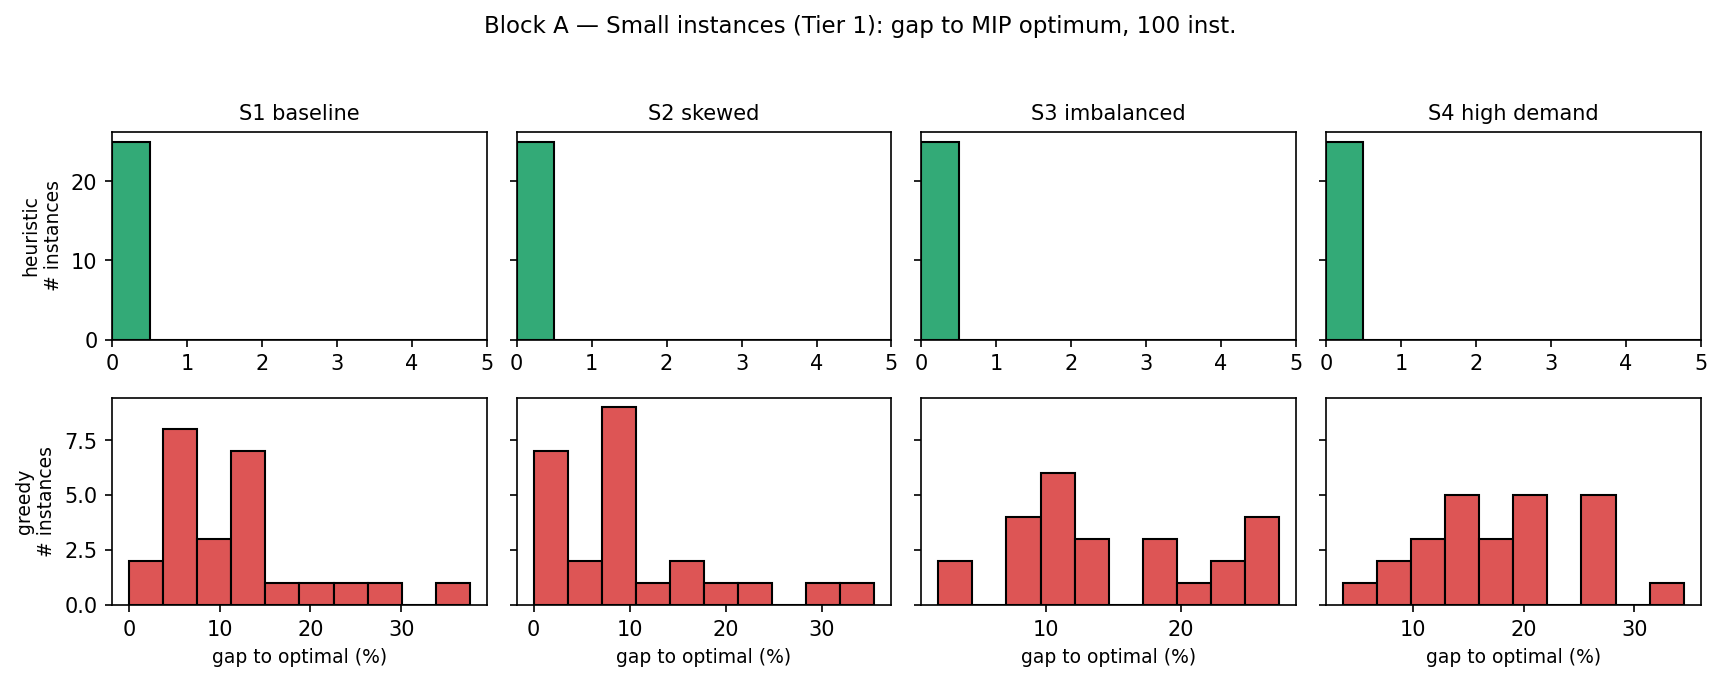
\includegraphics[width=\linewidth]{hist_blockA.png}
    \caption{Block A — gap to MIP optimum (100 inst.). \emph{Top:} heuristic is at $0\,\%$ on every instance. \emph{Bottom:} greedy has a wide right tail.}
\end{figure}

\begin{figure}[H]
    \centering
    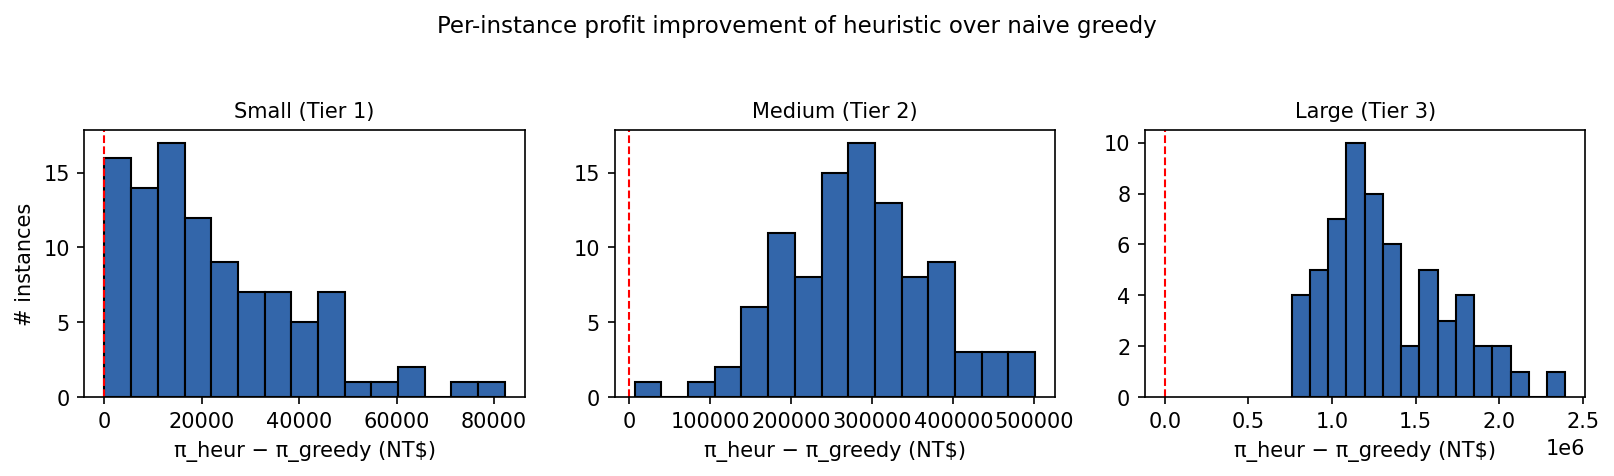
\includegraphics[width=\linewidth]{problem4_improvement.png}
    \caption{Per-instance profit advantage of the heuristic over the naive greedy, in NT\$, by block. \emph{All 260 bars are strictly right of zero}: the heuristic beats the greedy on every single random instance, with a margin that scales from $\sim\!10^4$ at Tier 1 to $\sim\!10^6$ at Tier 3.}
\end{figure}

\subsection{Conclusion and methodological caveat}

We tested every tier of the algorithm: at small scale it provably matches the optimum on $100/100$ instances; at medium and large scale, where no licence will solve the MILP, it dominates a plausible naive policy on \emph{every} one of the 160 additional instances with very small variance. The chief limitation is methodological: the LP relaxation is the only upper bound that scales, and it is loose for supply-constrained scenarios, so the reported $27$--$50\,\%$ gap-to-UB in Blocks B/C overstates the true distance to $\pi^{\ast}$ (the same phenomenon is observed and discussed by Tran et al.~\cite{tran2016} in their own large-instance experiments). The share-vs-greedy column and the dollar histogram are immune to this looseness and show a consistent advantage. We therefore submit the algorithm with reasonable confidence in instances 6--20.


\begin{thebibliography}{1}
\bibitem{tran2016} T.~T. Tran, A.~Araujo, and J.~C. Beck. Decomposition methods for the parallel machine scheduling problem with setups. \emph{INFORMS Journal on Computing}, 28(1):83--95, 2016.
\end{thebibliography}

\end{document}
